В данном разделе опишем разработанное программное обеспечение, с помощью
которого было проведено тестирование, данные, на которых проводилось
тестирование, а также представим и проанализируем полученные результаты.
\section{Описание программного обеспечения}
Программное обеспечение было написано на языке программирования
C++ по стандарту C++-11 под ОС Ubuntu. Сборка проекта осуществлялась
с помощью Cmake, использовался компилятор GNU.

Программное обеспечение работает с исходными данными,
данными о пользователях и объектах, которые хранятся в базе данных.
Пользователь исходного кода может сделать некоторые дополнения и
использовать другую базу данных. Класс подключения к базе создается
с помощью фабрики объектов.
Базовым классом, представляющим эту фабрику, является класс
ConnectionFactory, который имеет чистый виртуальный (pure virtual)
метод create и описан в файле db/connection-pool/ConntectionPool.h.
Пользователь должен сформировать собственную фабрику, класс которой
будет являться дочерним классом класса ConnectionFactory и которая
будет создавать объекты-коннекторы к конкретной базе.
Фабрика объектов-коннекторов создает объекты типа
std::shared\_ptr<Connection>, для которого определены чистые виртуальные методы
query и exec.
В разработанном
программном обеспечении данные хранились в базе MySql, поэтому был
создан класс MySQLConnectionFactory, в параметры конструктора которого
передаются параметры подключения к базе: хост, имя базы, логин и
пароль. В этом классе перегружен метод create, в теле которого
создается новое подключение к базе данных MySql, используя те
параметры, что были переданы в конструктор класса
MySQLConnectionFactory. Подключение происходит с помощью библиотеки
cppconn. Фабрика MySQLConnectionFactory создает объекты-коннекторы
типа MySQLConnection, в котором определены методы exec и query.
Таким образом, пользователь должен объявить два класса:
наследника класса ConnectionFactory и наследника класса Connection.
Фабрика, с помощью которой будет осуществляться создание объектов-коннекторов
и тип объектов коннекторов являются шаблонными параметрами класса
DbPoolGeneral, описанного в файле db/dbPool.h. Пользователю нужно
лишь указать имена этих параметров в определении typedef в конце файла,
как это сделано в текущем проекте:
\begin{verbatim}
	typedef DbPoolGeneral<
		active911::MySQLConnection,
		active911::MySQLConnectionFactory>

		DbPool;
\end{verbatim}
При использовании других баз и коннекторов нужно также внести изменения в файл
db/CmakeLists.txt и указать, какие библиотеки используются.

Интерфейсом пользователя программного обеспечения является командная
строка, в которой пользователь указывает параметры запуска.
Параметры запуска программы делятся на несколько логических групп,
а каждой группе принадлежит некоторое множество параметров:

\begin{itemize}
	\item параметры модели:
	\begin{itemize}
		\item $sim$ --- выбор функции, которая будет использоваться в качестве
			меры сходства. Реализованы следующие функции и соответствующие им
			имена параметров:
			\begin{itemize}
				\item $cos$ --- косинус угла между контами-векторами;
				\item $pearson$ --- коэффициент корреляции Пирсона;
				\item $hamming$ --- обобщенное расстояние Хэмминга.
			\end{itemize}
		\item $uidelta$ --- пороговое значение, которое соответствует
			$\Delta_{\R}$
		\item $delta$ --- пороговое значение меры сходства, соответствует
			$\Delta_u$ или $\Delta_i$.
	\end{itemize}
	\item параметры задачи:
	\begin{itemize}
		\item $N$ --- число объектов при решении задачи $topN$;
		\item $task$ --- решаемая задача. Либо параметр равен $p$, либо $topn$;
		\item $neighn$ --- число соседей, которые войдут в кластер;
		\item $sltn$ --- способ решения задачи. Реализованы следующие способы
			решения, которые может выбрать пользователь:
			\begin{itemize}
				\item $std$ --- стандартное решение задач методами коллаборативной
					фильтрации;
				\item $linear$ --- решение задачи $topN$ линейным поиском в нечеткой
					модели;
				\item $rnd$ --- случайное решение;
				\item $direct$ --- прямое вычисление $\rho(u_a, i)$, то есть
					решение задачи прогнозирования в нечеткой модели.
			\end{itemize}
	\end{itemize}
	\item функциональные параметры:
		\begin{itemize}
			\item $resplit$ --- опциональный параметр.опциональный параметр.
				Если он указан в командной строке, тогда произойдет разбиение
				исходных данных на обучающее и тестовое множество;
			\item $eval$ --- если параметр указан, то произойдет оценка
				качества и результаты сохранятся в соответствующей базе;
			\item $split\_alg$ --- алгоритм разбиения исходных данных на
				обучающее и тестовое множество. Возможны следующие варианты:
				\begin{itemize}
					\item $std$ --- стандартное разбиение, которое производится
						в случайном порядке;
					\item $div$ --- от diverse. Алгоритм формирует данные для
						каждого пользователя так,
						что в обучающем множестве находятся такие объекты между
						которыми и объектами тестового множества не выполняется
						отношение близости, если это возможно.
				\end{itemize}
			\item $split\_pcnt$ --- процент исходный данных, который войдет в
				обучающее множество;
			\item $calc$ --- если параметр указан, то будет произведено решение
				задачи --- если параметр указан, то будет произведено решение
				задачи;;
			\item $truncate$ --- очищение базы данных. Можно очистить один из
				четырех типов баз:
				\begin{itemize}
					\item $train$ --- обучающие данные;
					\item $test$ --- тестовые данные;
					\item $eval$ --- результаты оценки качества;
					\item $rslt$ --- результирующее множество.
				\end{itemize}
				Конкретное же имя базы формируется так:
				\begin{itemize}
					\item type + postfix, где type $\in \{eval, rslt\}$, postfix
						=
					$task$ + \_ + $sltn$ + \_ + $sim$ + \_ + $uidelta$ + \_ $delta$ +
					\_ $split$ + \_ + $split\_pcnt$ + $neighn$, где $task$ и
						т.д. конкретные значения указанных параметров, а знак +
						означает конкатеннацию строк;
					\item type + \_ + $task$ + \_ + $split\_pcnt$ +
						$split\_alg$,
						где type $\in \{train, test\}$, $task$ и т.п.
						означает конкретное значение соответствующего типа, указанного в
						командной строке.
				\end{itemize}

		\end{itemize}
\end{itemize}

Таким образом, пользователь с помощью командной строки
может запустить программу на выполнение следующих задач:
решить задачу при использовании различных параметров,
очистить базу данных, произвести расчет
оценки качества и разбить исходное множество на тестовое и обучающее.

Приведем несколько основных примеров запусков программы.

\begin{figure}[H]
	\caption{Пример запуска решения задачи $topN$ в ООМ}
	\label{pic:ex-topn-cos}
	\begin{center}
  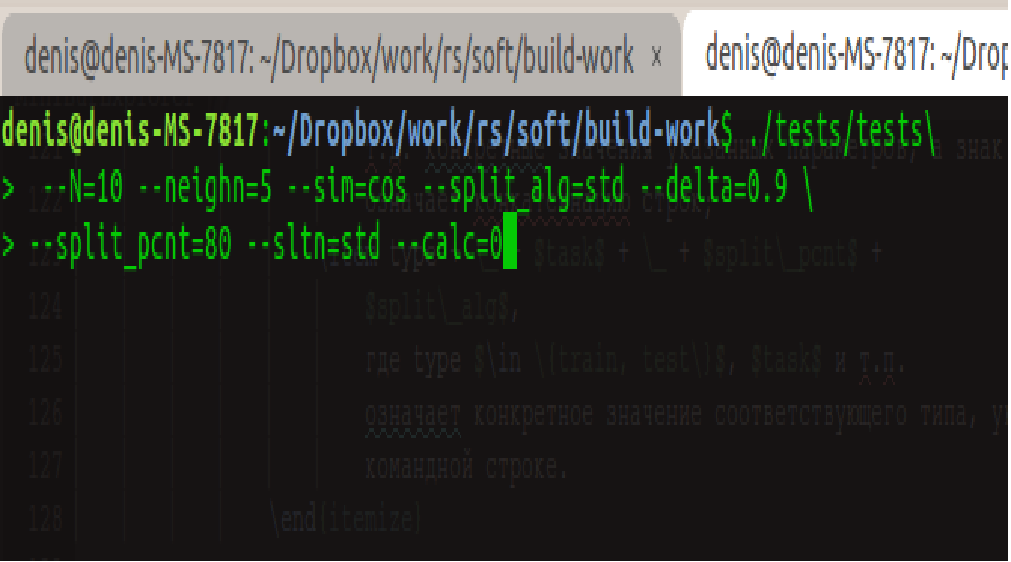
\includegraphics[width=7in,height=3in]{pics/examples/topn-cos.png}
\end{center}
\end{figure}

Пример запуска решения задачи $topN$ в ООМ стандартным
алгоритмом (\ref{alg:topn-solve-ors}) со следующими параметрами
\begin{itemize}
	\item $N=10$;
	\item мера сходства --- косинус;
	\item $\Delta_i = 0,9$;
	\item стандартное разбиение исходного множества данных на обучающее и
		тестовое множество;
	\item в обучающее множество входит 80\% исходных данных;
\end{itemize}
представлен на рисунке <<Пример запуска решения задачи $topN$ в ООМ>> (\ref{pic:ex-topn-cos}).

Пример запуска решения задачи $topN$ в нечеткой модели стандартным
алгоритмом (\ref{alg:topn-solve-ors}) со следующими параметрами:
\begin{itemize}
	\item $N=10$;
	\item $\Delta_i = 0,1$;
	\item стандартное разбиение исходного множества данных на обучающее и
		тестовое множество;
	\item в обучающее множество входит 80\% исходных данных;
\end{itemize}
представлен на рисунке <<Пример запуска решения задачи $topN$ в нечеткой модели при
	использовании $\Pi_C$>> (\ref{pic:ex-topn-hamming}).

\begin{figure}[H]
	\caption{Пример запуска решения задачи $topN$ в нечеткой модели при
	использовании $\Pi_C$}
	\label{pic:ex-topn-hamming}
	\begin{center}
  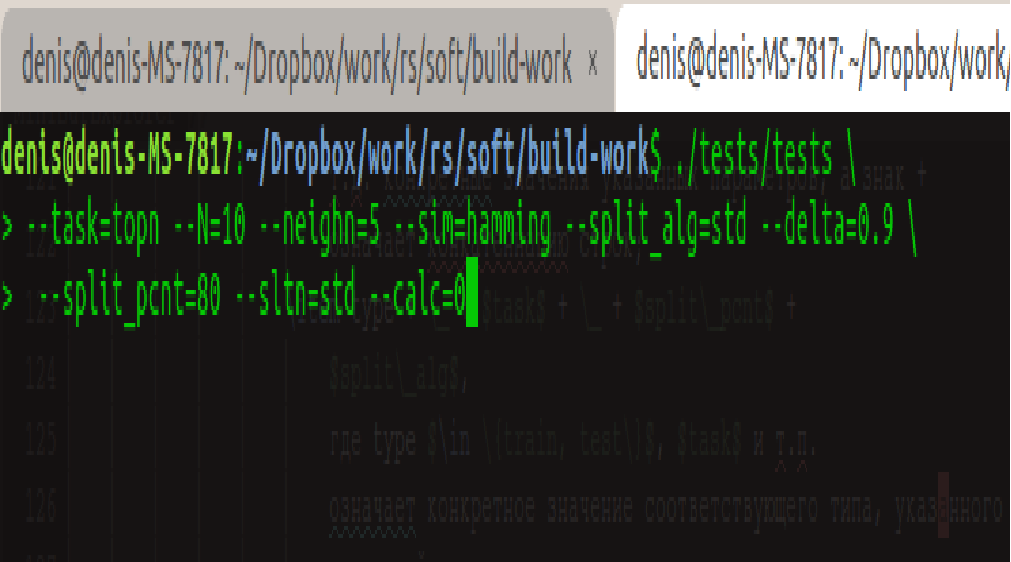
\includegraphics[width=7in,height=3in]{pics/examples/topn-hamming.png}
\end{center}
\end{figure}

Пример запуска решения задачи $topN$ в нечеткой модели
при использовании алгоритма линейного поиска (\ref{alg:fuz-topn}) со следующими
параметрами:
\begin{itemize}
	\item $N=10$;
	\item $\varepsilon_{\R} = 0,9$;
	\item стандартное разбиение исходного множества данных на обучающее и
		тестовое множество;
	\item в обучающее множество входит 80\% исходных данных;
\end{itemize}
представлен на рисунке <<Пример запуска решения задачи $topN$ в нечеткой модели при
	использовании $\Pi_f$>> (\ref{pic:ex-topn-fuz}).

\begin{figure}[H]
	\caption{Пример запуска решения задачи $topN$ в нечеткой модели при
	использовании $\Pi_f$}
	\label{pic:ex-topn-fuz}
	\begin{center}
	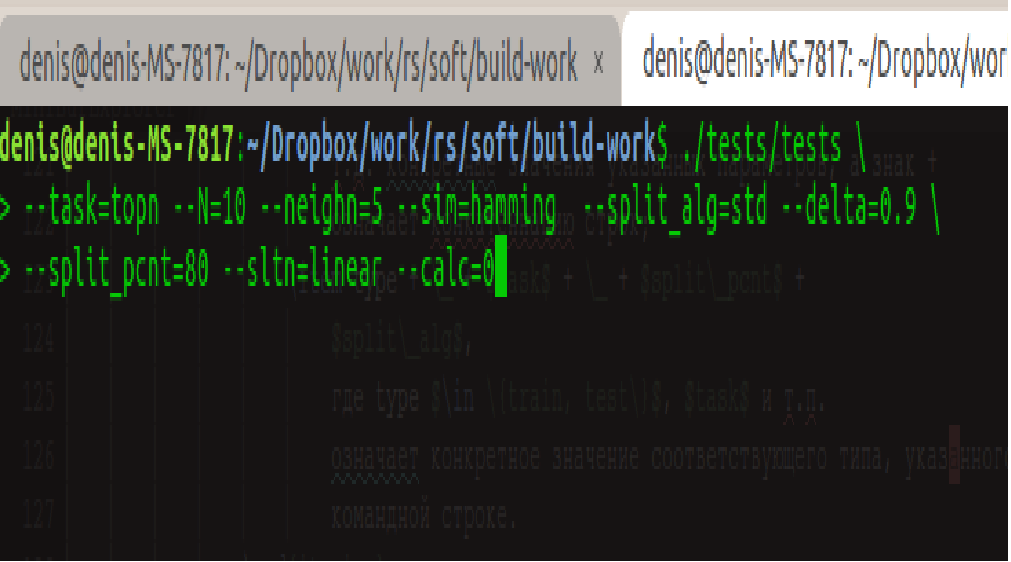
\includegraphics[width=7in,height=3in]{pics/examples/topn-fuz.png}
\end{center}
\end{figure}
%%%%%%%%%%%%%%%%%%%%%%%% p
Пример запуска решения задачи прогнозирования в CОМ стандартным
алгоритмом (\ref{alg:p-srs}) со следующими параметрами
\begin{itemize}
	\item мера сходства --- коэффициент корреляции Пирсона;
	\item $\Delta_u = 0,9$;
	\item стандартное разбиение исходного множества данных на обучающее и
		тестовое множество;
	\item в обучающее множество входит 80\% исходных данных;
\end{itemize}
представлен на рисунке <<Пример запуска решения задачи прогнозирования в СОМ>> (\ref{pic:ex-p-srs}).

\begin{figure}[H]
	\caption{Пример запуска решения задачи прогнозирования в СОМ}
	\label{pic:ex-p-srs}
	\begin{center}
  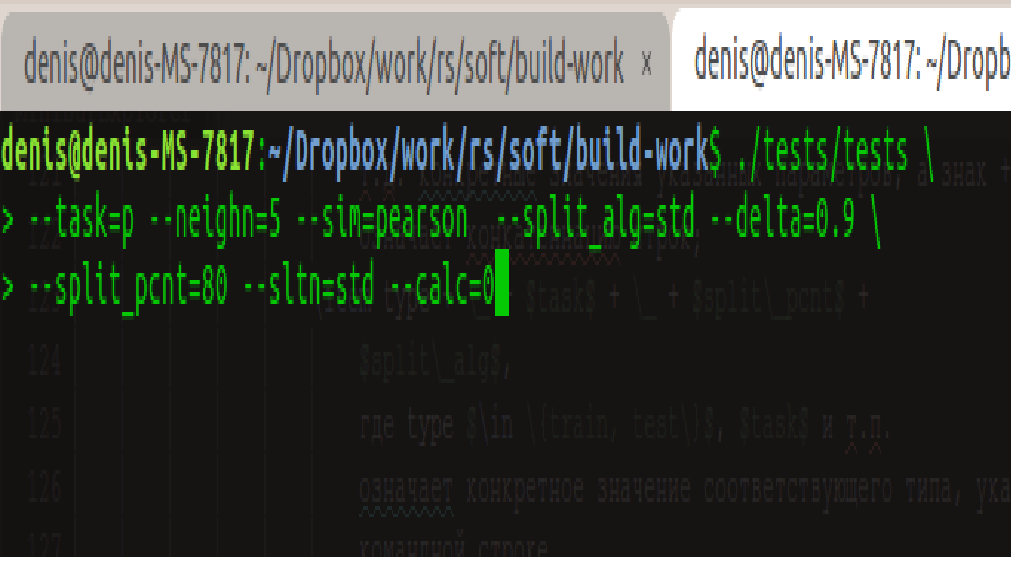
\includegraphics[width=7in,height=3in]{pics/examples/p-pearson.png}
\end{center}
\end{figure}

Пример запуска решения задачи прогнозирования в нечеткой модели стандартным
алгоритмом (\ref{alg:p-srs}) со следующими параметрами:
\begin{itemize}
	\item $\Delta_u = 0,1$;
	\item в обучающее множество входит 80\% исходных данных;
\end{itemize}
\begin{figure}[H]
	\caption{Пример запуска решения задачи прогнозирования в нечеткой модели при
	использовании $\Pi_C$}
	\label{pic:ex-p-srs-hamming}
	\begin{center}
  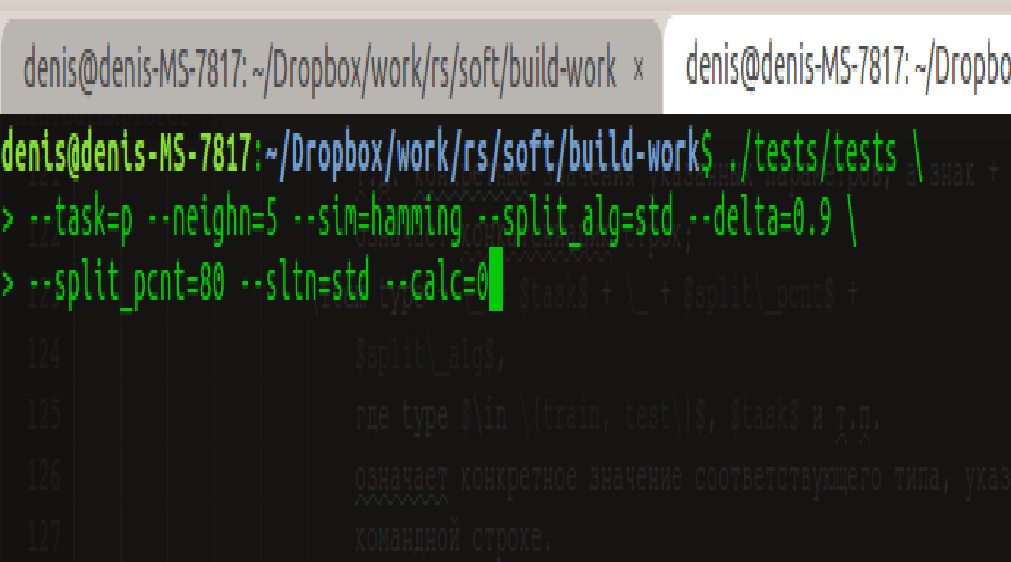
\includegraphics[width=7in,height=3in]{pics/examples/p-hamming.png}
\end{center}
\end{figure}
представлен на рисунке <<Пример запуска решения задачи прогнозирования в нечеткой модели при
	использовании $\Pi_C$>> (\ref{pic:ex-p-srs-hamming}).

Пример запуска решения задачи прогнозирования в нечеткой модели
алгоритмом нечеткой модели (\ref{alg:fuz-p}) со следующими параметрами:
\begin{itemize}
	\item $\varepsilon_{\R} = 0,9$;
	\item стандартное разбиение исходного множества данных на обучающее и
		тестовое множество;
	\item в обучающее множество входит 80\% исходных данных;
\end{itemize}
\begin{figure}[H]
	\caption{Пример запуска решения задачи прогнозирования в нечеткой модели при
	использовании $\Pi_f$}
	\label{pic:ex-p-srs-fuz}
	\begin{center}
  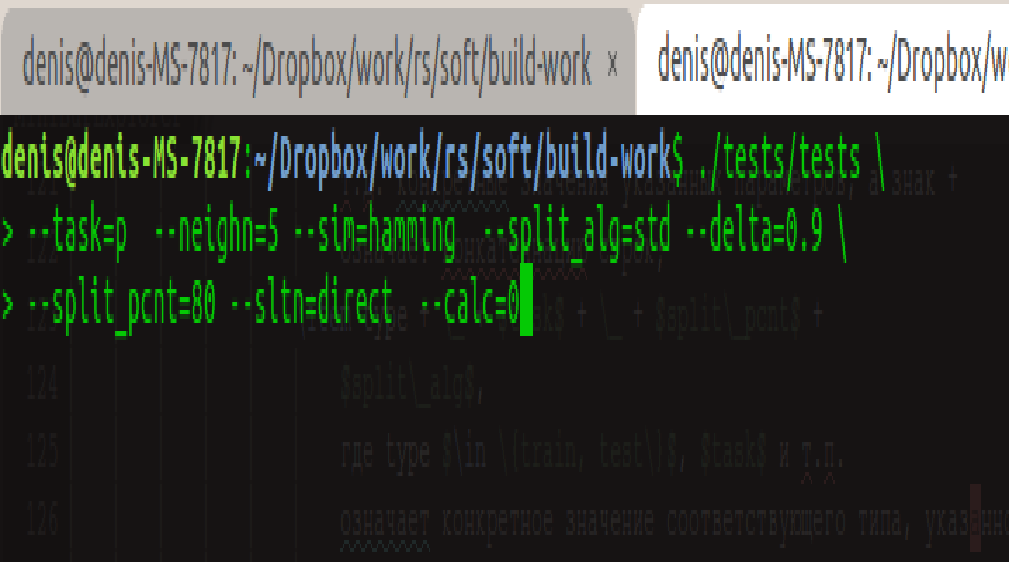
\includegraphics[width=7in,height=3in]{pics/examples/p-fuz.png}
\end{center}
\end{figure}
представлен на рисунке <<Пример запуска решения задачи прогнозирования в нечеткой модели при
	использовании $\Pi_f$>> (\ref{pic:ex-p-srs-hamming}).

%%%%%%%%%%%%%%%%%%%%
Пример очистки таблиц, в которых находятся результаты решения и оценки качества
решения задачи $topN$ в нечеткой модели представлен на рисунке <<Пример очистки
таблицы результатов и таблицы со значениями оценок качества>>.
(\ref{pic:truncate}).
\begin{figure}[H]
	\caption{Пример очистки таблицы результатов и таблицы со значениями оценок качества}
	\label{pic:truncate}
	\begin{center}
  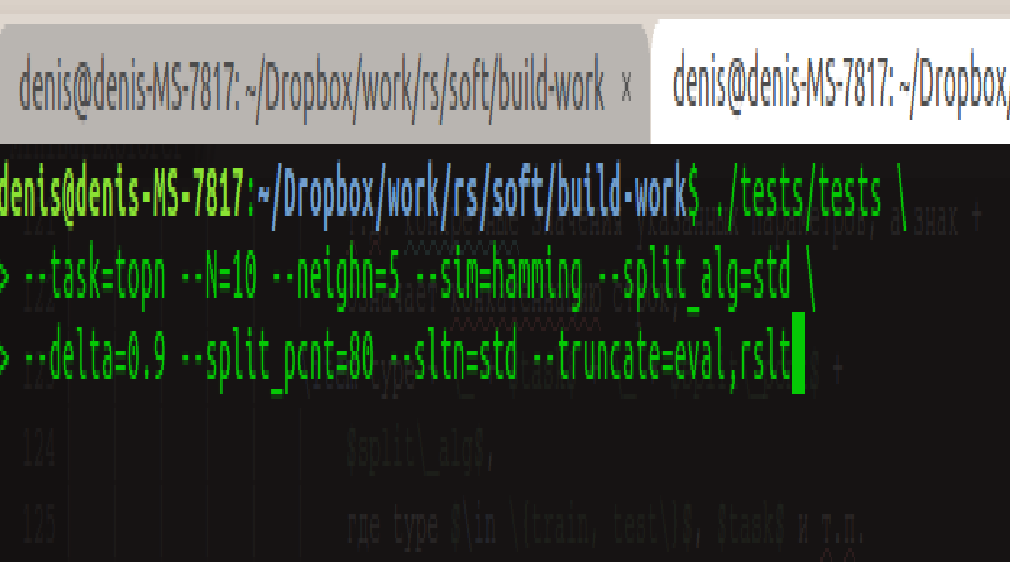
\includegraphics[width=7in,height=3in]{pics/examples/truncate.png}
\end{center}
\end{figure}

Пример вывода значений $P, AveP, NDCG$ при решении задачи $topN$ в нечеткой
модели при применении $\Pi_O$ представлен на рисунке <<Пример запуска программного обеспечения для вывода средних значений оценок
качества>> (\ref{pic:eval}).
\begin{figure}[H]
	\caption{Пример запуска программного обеспечения для вывода средних значений оценок
качества}
\label{pic:eval}
	\begin{center}
  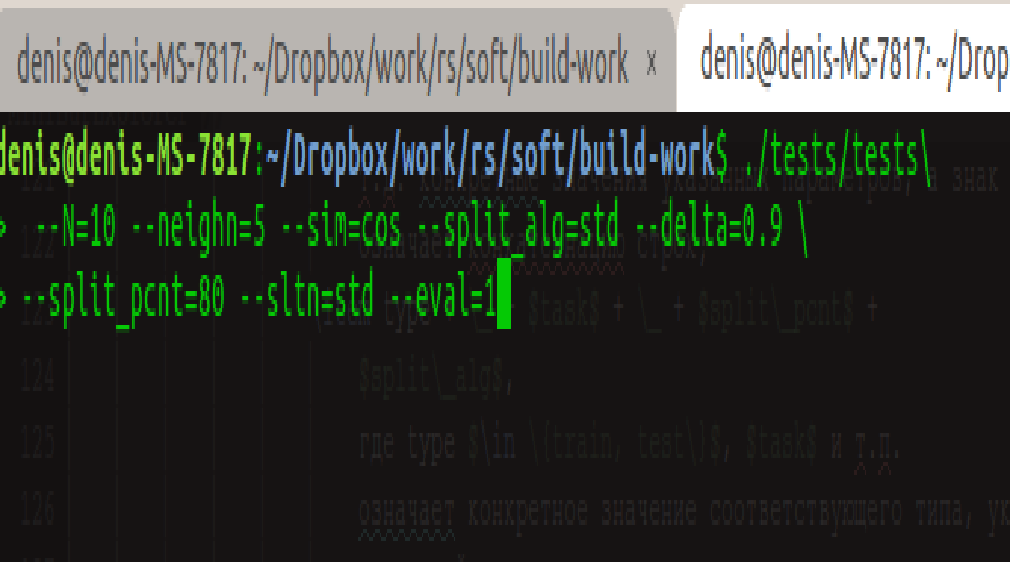
\includegraphics[width=7in,height=3in]{pics/examples/eval.png}
\end{center}
\end{figure}

Пример разбиения множества исходных данных на обучающее множество и тестовое
при применении стандартного алгоритма в пропорции 80 к 20 соответственно
представлен на рисунке <<Пример запуска программного обеспечения для формирования обучающего и тестового
множества при использовании разбиения 80 к 20 случайным образом (стандартное
разбиение)>> (\ref{pic:resplit}).
\begin{figure}[H]
	\caption{Пример запуска программного обеспечения для формирования обучающего и тестового
множества при использовании разбиения 80 к 20 случайным образом (стандартное
разбиение)}
\label{pic:resplit}
	\begin{center}
  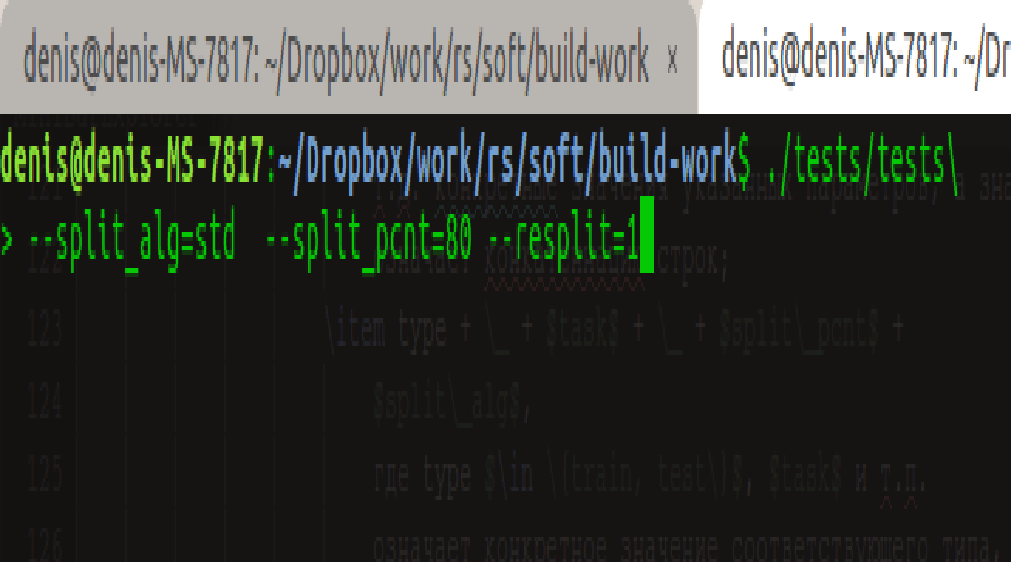
\includegraphics[width=7in,height=3in]{pics/examples/resplit.png}
\end{center}
\end{figure}
